\documentclass{article}
\usepackage[a4paper, margin=1in]{geometry}
\usepackage{graphicx} 
\usepackage{amsmath}
\usepackage{amssymb}
\usepackage{pgfplots}
\pgfplotsset{compat=1.18}
\usepackage{enumitem}

\title{\vspace{-2cm} \textbf{POE Answer Key \\ Semester II 2024-2025}}
\begin{document}
\date{}
\maketitle
\vspace{-1.5cm}
\noindent\hrulefill
\section*{Part A}
\begin{enumerate}
    \item 
        Input the given values in equation 
        \[
        Q_d^A = 40  - 0.02(20) + 0.9(8) = 46.8
        \]
    \item 
        Given
        $x$ = 3,
        $y$ = 2 $\Rightarrow$
        $U = (3)^2\times2 = 18$
    \item
        Price Elasticity of Demand is given by 
        \[\frac{\text{\%change in quantity demanded}}{\text{\%change in price}}\]
        $\epsilon_p$ = -20/40 = -0.5
    \item 
        The producer surplus per unit is the difference between the market price and the minimum price the producer is willing to accept. \\
        $\therefore$ Producer Surplus per unit = \$25 - \$15 = \$10
    \item 
        Marginal Cost = \(\frac{dC}{dQ}\) = \(15Q^2 + 8 - \frac{1}{Q}\) \\
        Given Q=12, $MC$ = \$2167.92
    \item 
        Breaking even quantity $(Q_B)$ is given by 
        \[
        TFC + AVC \cdot Q_B = P \cdot Q_B
        \]
        i.e. TC = TR $\Rightarrow$ Solving this gives $Q_B$ = 8 units
    \item 
        At $eq^m$, $Q^d=Q^s$ $\Rightarrow$ P=45 and Q=7 
    \item 
        MC = \(\frac{dC}{dQ}\) = $2Q+6$ \\
        In perfect competition, $P=D=MR=\$10$ \\ 
        Profit maximizing condition $\Rightarrow$ MC = MR $\Rightarrow$ Q=2 units
    \item 
        Equilibrium Quantity $Q^* = 30$\\
        \text{Producer Surplus} = \(\frac{1}{2}\) $\times$ 30 $\times$ (20-5) = 225
    \item 
        X and Y are complementary goods. Cross Price Elasticity of demand is given by
        \[\frac{\text{\%change in quantity demanded of Y}}{\text{\%change in price of X}}\]
        $\epsilon_c$ = -0.8 $\Rightarrow$ \%change in quantity demanded of Y = -8\% \\
        Thus, the demand of Y decreases by 8\%
\end{enumerate}

\section*{Part B}
\begin{enumerate}
    \item
        Input value of $P_y$ and rearrange the terms to obtain the Inverse Demand Function
        \[
        P_x = 5 - 0.5Q_d
        \]
        $\therefore$ \text{Consumer Surplus} = \(\frac{1}{2}\) $\times$ (4-0) $\times$ (5-3) = 4
    \item 
        Price Elasticity of Demand is given by 
        \[
        \epsilon_p=\frac{dQ_A^d}{dP_A} \cdot \frac{P_A}{Q_A^d}
        \]
        $\epsilon_p$ = -0.02 $\times$ 196.8 = -3.936  
    \item 
        \text{Total Cost} = \text{Fixed Costs} + \text{Variable Costs} \\
        Substituting \( Q = 6 \) into the functions\\
        TVC = 1878, TC = 2178, TR = 2016 \\
        $Loss$ = TC - TR = 162 \\
        \text{Average Total Cost} = \(\frac{TC}{Q}\) = 363 \\
        Since \( TR > TVC \), the firm covers its variable costs and should continue operating in the short run.
    \item 
        $\epsilon_D$ = \(\frac{dQ^d}{dP} \cdot \frac{P}{Q^d}\) = -0.4, 
        $\epsilon_S$ = \(\frac{dQ^s}{dP} \cdot \frac{P}{Q^s}\) = 0.5
        \begin{align}
        Q^d = m_1P+c_1 \\
        Q^s = m_2P+c_2  
        \end{align}
        Substituting $P=5, Q^d = Q^s = 16$ \\ 
        $m_1$ = \(\frac{dQ^d}{dP}\) = -1.28 \\
        $m_2$ = \(\frac{dQ^s}{dP}\) = $1.6$ \\
        $c_1 = 22.4$ and $c_2 = 8$ \\
        $Q^d = -1.28P+22.4$ and $Q^s = 1.6P+8$
    \item 
        To find optimal consumption bundle $(x,y)$, the utility function must be maximized under the budget constraint
        \[
        4x+2y=40
        \]
        Condition for maximum utility is as follows 
        \[
        \frac{P_x}{P_y} = \frac{MU_x}{MU_y} 
        \]
        $MU_x$ = \(\frac{\partial U}{\partial x}\), $MU_y$ = \(\frac{\partial U}{\partial y}\)\\
        Solving this gives $y=2x$. Substituting this into the budget constraint gives x=5 $\Rightarrow$ y=10 \\
        $\therefore$ (5,10) is the optimum consumption bundle.
    \item 
        Accounting Cost = $55,000 + 25,000$ = \$80,000 \\
        Opportunity Cost = $120,000-55,000+30,000$ = \$95,000 \\
        Economic Cost = Accounting Cost + Opportunity Cost = \$175,000
    \item 
        Isocost Line is given by $20L+120K=4200$ and the optimal combination (L,K) which would maximize the company's production must satisfy the condition
        \[
        \frac{P_L}{P_K} = \frac{MP_L}{MP_K}
        \]
        $MP_L$ = \(\frac{\partial Q}{\partial L}\), $MP_K$ = \(\frac{\partial Q}{\partial K}\)\\
        Solving this gives \(\frac{K}{L}=\frac{2}{9}\). Substituting this into the isocost equation gives $L=90$ and $K=20$
    \item 
        When the inputs are scaled by a constant factor \( t > 1 \), the scaled production function becomes:
        \[
        F(tK, tL) = A (tK)^\alpha (tL)^\beta = t^{\alpha + \beta} A K^\alpha L^\beta = t^{\alpha + \beta} F(K,L)
        \]
        The type of returns to scale depends on the value of the exponent \( \alpha + \beta \)
        \begin{itemize}
            \item If \( \alpha + \beta = 1 \), constant returns to scale
            \[
            F(tK, tL) = tF(K, L)
            \]
            \item If \( \alpha + \beta > 1 \), increasing returns to scale
            \[
            F(tK, tL) > tF(K, L)
            \]
            \item  If \( \alpha + \beta < 1 \), decreasing returns to scale
            \[
            F(tK, tL) < tF(K, L)
            \]
        \end{itemize}
    \item 
        For a monopolist, D = AR $\neq$ MR \\
        TR=P$\times$Q $\Rightarrow$ $TR = 100Q-2Q^2$ \\
        $MR=\frac{d(TR)}{dQ} \Rightarrow MR=100-4Q$ \\
        $MC=\frac{d(TC)}{dQ} \Rightarrow MC=6Q$ \\
        Condition for profit maximization is 
        \[
        MR = MC
        \]
        Solving this gives $Q=10$ units and substituting this back into the monopolist's demand curve gives $P = \$80$ \\
    \item
        The inverse demand and inverse supply functions are 
        \begin{align}
        P=8-4Q^d \tag{1} \\
        P=5+2Q^s \tag{2}
        \end{align}
        A price floor above the equilibrium price creates surplus in the market and can be plotted as shown \\
        \begin{center}
        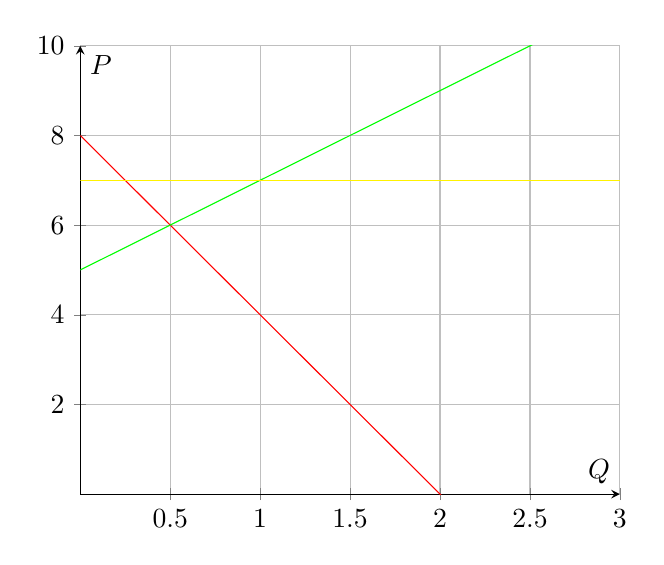
\begin{tikzpicture}
            \begin{axis}[
                axis lines=middle,
                xlabel={$Q$},
                ylabel={$P$},
                xmin=0, xmax=3,
                ymin=0, ymax=10,
                grid=major,
            ]
                \addplot[color=red, domain=0:7, samples=100] {8 - 4*x};
                \addplot[color=green, domain=0:7, samples=100 ] {2*x + 5};
                \addplot[color=yellow, domain=0:7, samples=100] {7};
            \end{axis}
        \end{tikzpicture}
        \end{center}
        \begin{itemize}
        \item Consumer Surplus = \(\frac{1}{2}\) $\times$ (0.25-0) $\times$ (8-7) = 0.125 \\
        \item Producer Surplus = \(\frac{1}{2}\) $\times$ [(7-5)+(7-5.5)] $\times$ (0.25-0) = 0.4375 \\
        \item Deadweight Loss = \(\frac{1}{2}\) $\times$ (7-5.5) $\times$ (0.5-0.25) = 0.1875 \\
        \end{itemize}
\end{enumerate}
\section*{Part C}
\begin{enumerate}
    \item 
        \textbf{Initial Basket} \\
        Budget Constraint is given by $5A+8B=120$ $\Rightarrow$
        $\frac{MU_A}{MU_B} = \frac{p_A}{p_B} \Rightarrow A=\frac{16}{5}B$ \\
        Putting this back into the constraint, we get $A=16$ and $B=5 \Rightarrow (16,5)$ \\
        \textbf{Final Basket} \\
        Budget Constraint is given by $3A+8B=120$ $\Rightarrow$
        $\frac{MU_A}{MU_B} = \frac{p_A^{'}}{p_B} \Rightarrow A=\frac{16}{3}B$ \\
        Putting this back into the constraint, we get $A=26.67$ and $B=5 \Rightarrow (26.67,5)$ \\
        \textbf{Decomposition Basket} \\
        This basket will have same utility as the initial basket but will follow the tangency condition with new prices. Initial utility = $4(16)^2(5)=5120$ and $A=\frac{16}{3}B$ \\
        Therefore, $(4)(\frac{16}{3}B)^2B = 5120 \Rightarrow B=3.56$ and $A=18.97 \Rightarrow (18.97,3.56)$
        \begin{enumerate}[label=(\roman*)]
            \item Income Effect on A = final - decomposition basket values of A = 7.7
            \item Substitution Effect on B = decomposition - initial basket values of B = -1.44
        \end{enumerate}        
    \item 
        $TR=P\cdot Q \Rightarrow TR=30Q-3Q^2 \Rightarrow MR = 30-6Q$ \\
        $MC = 6Q$ \\
        Socially optimal level would be the point where $MC=D$, where D is the monopoly's demand curve $\Rightarrow 6Q=30-3Q \Rightarrow Q=3.33$ and $P=\$20$.
        \begin{center}
        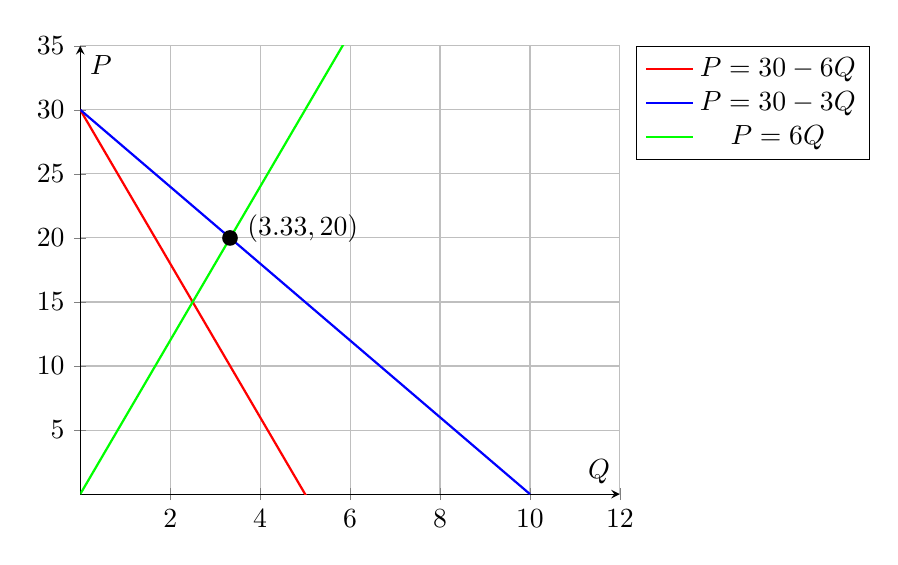
\begin{tikzpicture}
            \begin{axis}[
                axis lines=middle,
                xlabel={$Q$},
                ylabel={$P$},
                xmin=0, xmax=12,
                ymin=0, ymax=35,
                grid=major,
                xtick={0,2,4,6,8,10,12}, 
                ytick={0,5,10,15,20,25,30,35},
                legend pos=outer north east
            ]
            \addplot[red, thick, domain=0:10] {30 - 6*x};
            \addlegendentry{$P=30-6Q$}
            \addplot[blue, thick, domain=0:10] {30 - 3*x};
            \addlegendentry{$P=30-3Q$}
            \addplot[green, thick, domain=0:10] {6*x};
            \addlegendentry{$P=6Q$}
            \node[fill=black, circle, inner sep=2pt] at (axis cs:3.33,20) {};
            \node[anchor=west] at (axis cs:3.5,20.7) {$(3.33,20)$};
            \end{axis}
        \end{tikzpicture}
        \end{center}
        Social cost of monopoly is simply the deadweight loss generated because of monopoly producing where $MC=MR$ instead. Therefore, \\
        $\text{Social Cost} = \frac{1}{2} \times (22.5-15) \times (3.33-2.5) = 3.125$
    \item 
        Inverse demand and supply functions would be 
        \begin{align}
            P=40-\frac{1}{5}Q^d \tag{1} \\
            P=\frac{1}{3}Q^s + 20 \tag{2}
        \end{align}
        A \$10 per unit tax shifts the supply curve upwards by 10 units. Thus the new inverse supply function is given by $P=\frac{1}{3}Q^s + 30$ \\
        \begin{center}
            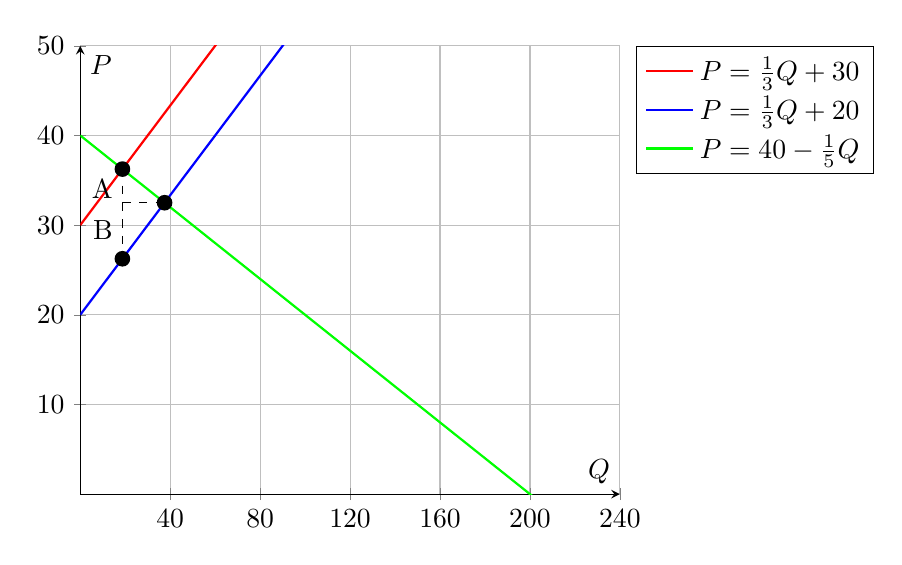
\begin{tikzpicture}
                \begin{axis}[
                    axis lines=middle,
                    xlabel={$Q$},
                    ylabel={$P$},
                    xmin=0, xmax=240,
                    ymin=0, ymax=50,
                    xtick={40,80,120,160,200,240},
                    ytick={10,20,30,40,50},
                    grid=major,
                    legend pos=outer north east
                ]
                \addplot[domain=0:250, red, thick] {(1/3)*x + 30};
                \addplot[domain=0:250, blue, thick] {(1/3)*x + 20};
                \addplot[domain=0:250, green, thick] {40 - (1/5)*x};
                \addlegendentry{$P = \frac{1}{3}Q + 30$};
                \addlegendentry{$P = \frac{1}{3}Q + 20$};
                \addlegendentry{$P = 40 - \frac{1}{5}Q$};
            
                % Intersection points
                \node[fill=black, circle, inner sep=2pt] at (axis cs:37.5,32.5) {};
                \node[fill=black, circle, inner sep=2pt] at (axis cs:18.75,36.25) {};
                \node[fill=black, circle, inner sep=2pt] at (axis cs:18.75,26.25) {};
                % Labels for segments
                \draw[dashed] (axis cs:18.75,36.25) -- (axis cs:18.75,32.5);
                \draw[dashed] (axis cs:18.75,32.5) -- (axis cs:18.75,26.25);
                \node[left] at (axis cs:18.75,34) {A};
                \node[left] at (axis cs:18.75,29.5) {B};
                \draw[dashed] (axis cs:18.75,32.5) -- (axis cs:37.5,32.5);
                \end{axis}
            \end{tikzpicture}
        \end{center}
        A per unit tax shifts the equilibrium from $(37.5,32.5)$ to $(18.75,36.25)$. The producers charge \$36.25 for the product but only keep \$26.25 with them due to tax. The burden on consumers and producers is given by vertical distances A and B respectively as shown above.  
        \begin{enumerate}[label=(\roman*)]
            \item Consumer burden = \$3.75
            \item Producer burden = \$6.25
        \end{enumerate}        
    \item
        Inverse demand function is $P=20-\frac{1}{5}Q \Rightarrow TR=PQ=20Q-\frac{1}{5}Q^2 \Rightarrow MR=20-\frac{2}{5}Q$\\
        When maximizing profits
        \[
        MC=MC_1=MC_2
        \]
        $Q=Q_1+Q_2$ where $Q_1 = \frac{1}{5}MC_1-2$ and $Q_2=\frac{1}{5}MC_2-3$\\
        Therefore $Q=\frac{2}{5}MC-5 \Rightarrow MC=\frac{5}{2}Q+\frac{25}{2}$ \\
        $MC=MR \Rightarrow \frac{5}{2}Q+\frac{25}{2} = 20-\frac{2}{5}Q \Rightarrow Q=2.59$ and $P=\$19.48$ \\
        $MC_1 = MC_2 = MC = 18.98$. Substitute this in each plant's marginal cost equation to obtain output level of each plant
        $\Rightarrow Q_1=1.796$ and $Q_2=0.796$
    \item 
        Since x and y are consumed in a fixed ratio i.e $\frac{x}{y} = \frac{3}{2}$, the utility obtained from any bundle (x,y) only changes when $(x,y)=k(3,2)$ i.e. the new bundle is a scalar multiple of the fixed consumption bundle. The consumer would be indifferent to other bundles, for example $U_{(3,2)} = U_{(4,2)}$ but $U_{(6,4)} > U_{(3,2)}$. This notion can be extended and the utility for any consumption bundle can be expressed as 
        \[
        U(x,y) = min(2x,3y)
        \]
        $U(x,y)=10$ will be a L shaped curve with vertex at $2x=3y=10 \Rightarrow x=5$ and $y=3.33$
        \begin{center}
        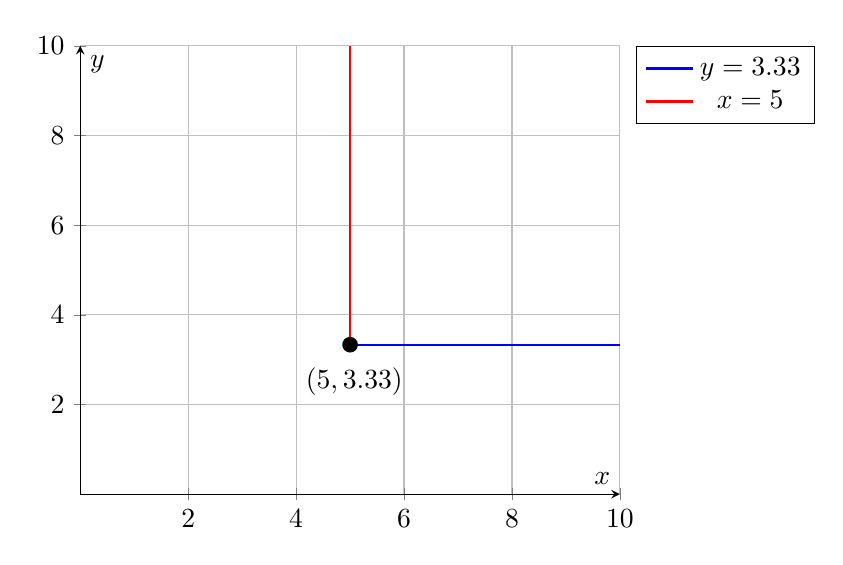
\begin{tikzpicture}
            \begin{axis}[
                axis lines=middle,
                xlabel={$x$},
                ylabel={$y$},
                xmin=0, xmax=10,
                ymin=0, ymax=10,
                grid=major,
                legend pos=outer north east
                ]
                \addplot[domain=5:10, blue, thick] {3.333};
                \addplot[red, thick] coordinates {(5,3.333) (5,10)};
                \addlegendentry{$y=3.33$};
                \addlegendentry{$x=5$};
                \node[fill=black, circle, inner sep=2pt] at (axis cs:5,3.333) {};
                \node[anchor=west] at (axis cs:4,2.5) {$(5,3.33)$};
            \end{axis}
        \end{tikzpicture}
        \end{center}        
    \item
        $MC=\frac{d(TC)}{dQ} \Rightarrow MC=2Q$ \\
        $TR=P\cdot Q = 180Q-2Q^2 \Rightarrow MR=180-4Q$ 
        \begin{center}
        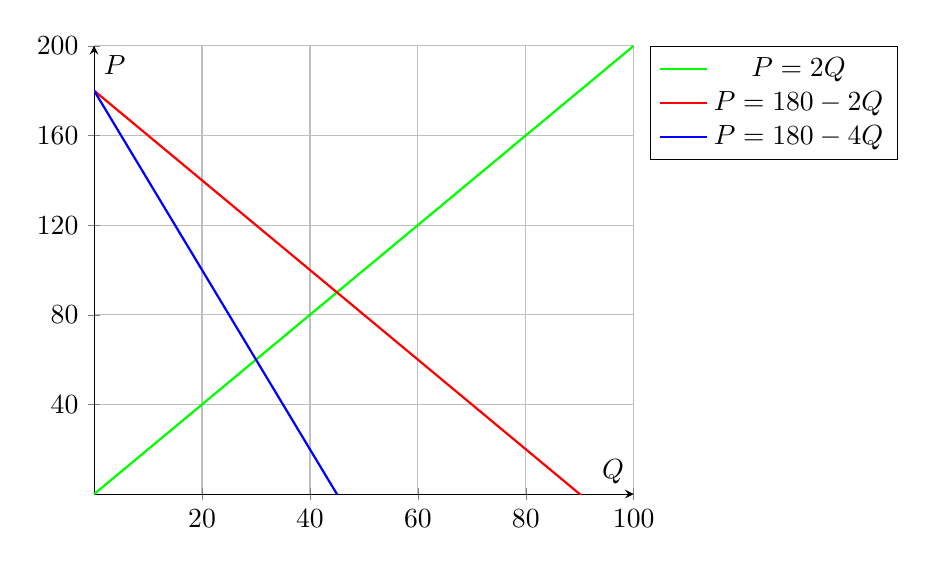
\begin{tikzpicture}
            \begin{axis}[
                axis lines=middle,
                xlabel={$Q$},
                ylabel={$P$},
                xmin=0, xmax=100,
                ymin=0, ymax=200,
                grid=major,
                xtick={0,20,40,60,80,100}, 
                ytick={0,40,80,120,160,200},
                legend pos = outer north east,
                ]
                \addplot[domain=0:100, green, thick] {2*x};
                \addlegendentry{$P=2Q$}
                \addplot[domain=0:160, red, thick] {180 - 2*x};
                \addlegendentry{$P=180-2Q$}
                \addplot[domain=0:160, blue, thick] {180 - 4*x};
                \addlegendentry{$P=180-4Q$}             
            \end{axis}
        \end{tikzpicture}
        \end{center}
        Initially, market was at perfect competition i.e producing at $AR=MC$ where P=90 and Q=45.
        \begin{itemize}
            \item Consumer Surplus = \(\frac{1}{2}\) $\times$ (180-90) $\times$ (45-0) = 2025 \\
            \item Producer Surplus = \(\frac{1}{2}\) $\times$ (90-0) $\times$ (45-0) = 2025 \\
            \item Deadweight Loss = 0 
        \end{itemize}
        Now market is monopolistic, producing at the quantity where $MC=MR$ i.e Q=30 and charging a price of P=120.
        \begin{itemize}
            \item Consumer Surplus = \(\frac{1}{2}\) $\times$ (180-120) $\times$ (30-0) = 900 \\
            \item Producer Surplus = \(\frac{1}{2}\) $\times$ [(120-0)+(120-60)] $\times$ (30-0) = 2700 \\
            \item Deadweight Loss = \(\frac{1}{2}\) $\times$ (120-60) $\times$ (45-30) = 450 
        \end{itemize}
        $\therefore \Delta CS=-1125$ , $\Delta PS=675$ , $\Delta DWL= 450$
    \item 
        A subsidy would decrease price of the good since the firm's costs decreased. The benefit distribution can be obtained by 
        \begin{align*}
            B_C = \frac{\epsilon_s}{\epsilon_d + \epsilon_s} \\
            B_P = \frac{\epsilon_d}{\epsilon_d + \epsilon_s}
        \end{align*}
        where $B_C$ and $B_P$ are the proportion of benefit to consumers and producers respectively (use absolute values of elasticity).
        \begin{align*}
            \text{Consumer Benefit} = B_C \times \text{Subsidy} \\
            \text{Producer Benefit} = B_P \times \text{Subsidy}
        \end{align*}
        Put in the values and solve $\Rightarrow$ CB=\$3/unit and PB=\$2/unit.
    \item 
        For optimal consumption bundle, 
        \[
        MRS=\frac{MU_x}{MU_y} = \frac{p_x}{p_y} \Rightarrow \frac{1}{x} = \frac{p_x}{p_y} \Rightarrow x^* = \frac{p_y}{p_x}
        \]
        Putting this back into the budget constraint, 
        \[
        M=p_x(\frac{p_y}{p_x}) + p_yy \Rightarrow y^* = \frac{M}{p_y} - 1
        \]
        $\therefore (x^*,y^*) = (\frac{p_y}{p_x},\frac{M}{p_y} -1)$ \\
        For $M\le p_y \Rightarrow y^*=0$ thus $x^*=\frac{M}{p_x}$, but for $M\ge p_y$ value of $x^* = \frac{p_y}{p_x}$, which is independent of M. Thus the graph of M against $x^*$ will look as shown below. 
        \begin{center}
        \begin{tikzpicture}
            \draw[->] (0,0) -- (5,0) node[right] {$x^*$};
            \draw[->] (0,0) -- (0,4.5) node[left] {$M$};
            \node[left] at (0,2) {$p_y$};
            \node[below] at (3,0) {$\frac{p_y}{p_x}$};
            \draw[thick] (0,0) -- (3,2);
            \draw[thick] (3,2) -- (3,4.5);
            \draw[dashed] (3,0) -- (3,2);
            \draw[dashed] (0,2) -- (3,2);
        \end{tikzpicture}
        \end{center}
        As income (M) increases, consumption of good x increases but after a point, the consumption remains constant despite further increase in income. An example of such a good would be salt. 
    \item 
        From Question 3, we know the graph looks like 
        \begin{center}
            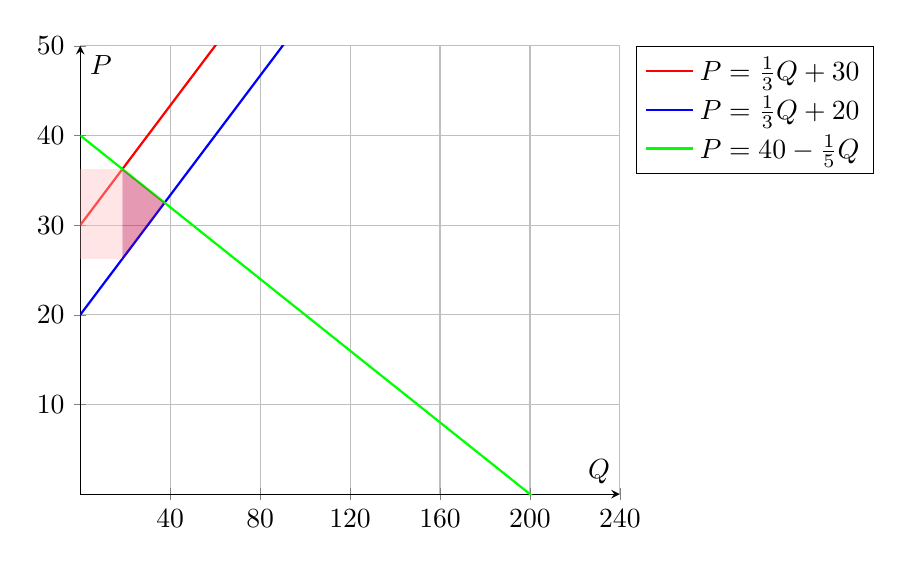
\begin{tikzpicture}
                \begin{axis}[
                    axis lines=middle,
                    xlabel={$Q$},
                    ylabel={$P$},
                    xmin=0, xmax=240,
                    ymin=0, ymax=50,
                    xtick={40,80,120,160,200,240},
                    ytick={10,20,30,40,50},
                    grid=major,
                    legend pos=outer north east
                ]
                \addplot[domain=0:250, red, thick] {(1/3)*x + 30};
                \addplot[domain=0:250, blue, thick] {(1/3)*x + 20};
                \addplot[domain=0:250, green, thick] {40 - (1/5)*x};
                \addlegendentry{$P = \frac{1}{3}Q + 30$};
                \addlegendentry{$P = \frac{1}{3}Q + 20$};
                \addlegendentry{$P = 40 - \frac{1}{5}Q$};
                \fill[pink, opacity=0.4] (axis cs:0,36.25) -- (axis cs:18.75,36.25) -- (axis cs:18.75,26.25) -- (axis cs:0,26.25) -- cycle;
                \fill[purple, opacity=0.4] (axis cs:18.75,36.25) -- (axis cs:18.75,26.25) -- (axis cs:37.5,32.5) -- cycle;
                \end{axis}
            \end{tikzpicture}
        \end{center}
        \begin{enumerate}[label=(\roman*)]
            \item Deadweight loss = $\frac{1}{2} \times (36.25-26.25) \times (37.5-18.75) = 93.75$
            \item Tax Revenue = $10 \times 18.75 = \$187.5$
        \end{enumerate}   
    \item 
        Budget Line is $2x+5y=10$ and let the maximum utility indifference curve be given by the equation $3x+4y=c$ where c is some constant.\\
        Since X and Y are perfect substitutes, consumer would spend all their income on the good with higher marginal utility per dollar. 
        \[
        \frac{MU_x}{P_x} = 1.5
        \]
        \[
        \frac{MU_y}{P_y} = 0.8
        \]
        Graphically, this implies optimal consumption bundle lies on the x intercept of the budget line. 
        \begin{center}
        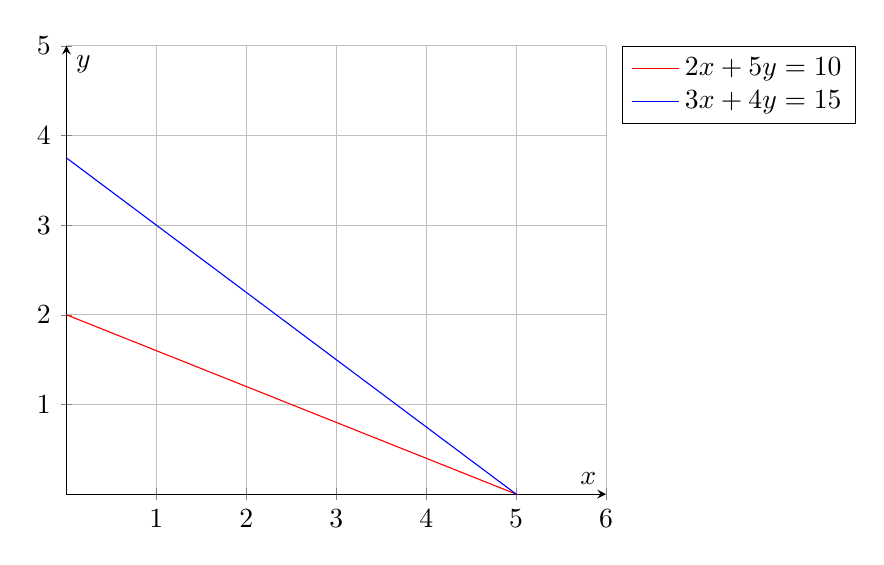
\begin{tikzpicture}
            \begin{axis}[
                axis lines = middle,
                xlabel = {$x$},
                ylabel = {$y$},
                xmin = 0, xmax = 6,
                ymin = 0, ymax = 5,
                legend pos = outer north east,
                grid = major
            ]
            \addplot[color=red, domain=0:7, samples=100] { (1 - 0.2*x) / 0.5 };
            \addlegendentry{$2x + 5y = 10$}
            \addplot[color=blue, domain=0:7, samples=100] { (15 - 3*x) / 4 };
            \addlegendentry{$3x + 4y = 15$}
            \end{axis}
        \end{tikzpicture}
        \end{center}
        From the budget constraint we have $2x+5(0)=10 \Rightarrow x=5$ \\
        Optimal consumption bundle is (5,0) and indifference curve is given by $3x+4y=15$
    \item 
        (b) Hint: P$\uparrow$ and Substitution Effect is -ve, Income Effect is -ve, Price (total) Effect is -ve
    \item 
        (c) Hint: P$\downarrow$ and Substitution Effect is +ve, Income Effect is -ve, Price (total) Effect is +ve
    \item
        (b) Hint: P$\downarrow$ and Substitution Effect is +ve, Income Effect is +ve, Price (total) Effect is +ve
    \item 
        $TR=P\cdot Q = 20Q-Q^2 \Rightarrow MR=20-2Q$ \\ 
        \textbf{Before tax} \\
        $MC=2Q$\\
        $MC=MR \Rightarrow Q^*=5$ \\
        $P^*=20-Q^*=\$15$ 
        \begin{center}
        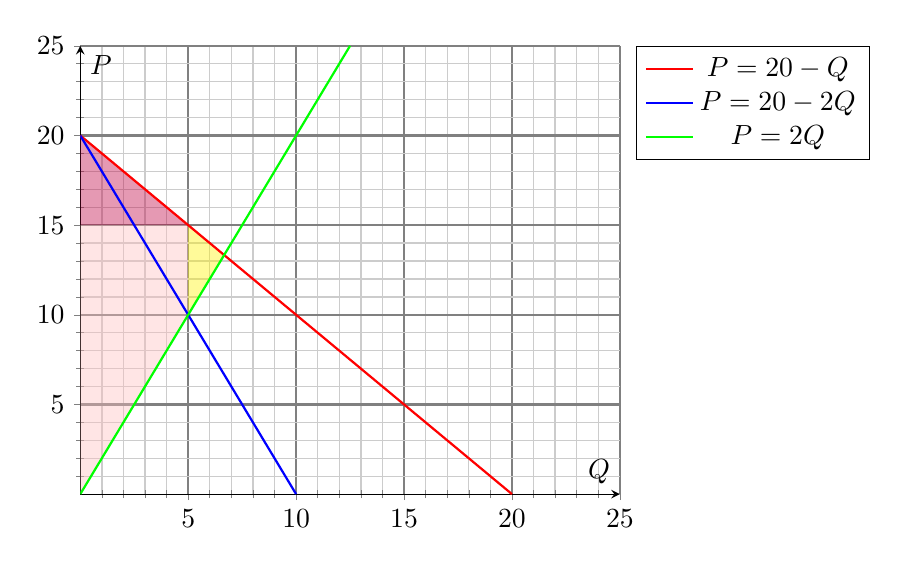
\begin{tikzpicture}
            \begin{axis}[
                axis lines=middle,
                xlabel={$Q$},
                ylabel={$P$},
                xmin=0, xmax=25,
                ymin=0, ymax=25,
                grid=both,
                minor tick num=4, 
                major grid style={line width=0.8pt,draw=black!50},
                minor grid style={line width=0.5pt,draw=black!20},
                legend pos=outer north east
            ]
            
            \fill[pink, opacity=0.4] (axis cs:0,15) -- (axis cs:5,15) -- (axis cs:5,10) -- (axis cs:0,0) -- cycle;
            
            \fill[purple, opacity=0.4] (axis cs:0,15) -- (axis cs:0,20) -- (axis cs:5,15) -- cycle;
            
            \fill[yellow, opacity=0.4] (axis cs:5,10) -- (axis cs:5,15) -- (axis cs:6.67,13.34) -- cycle;
            
            \addplot[red, thick, domain=0:20] {20 - x};
            \addlegendentry{$P=20-Q$}
            \addplot[blue, thick, domain=0:10] {20 - 2*x};
            \addlegendentry{$P=20-2Q$}
            \addplot[green, thick, domain=0:12.5] {2*x};
            \addlegendentry{$P=2Q$}
            \end{axis}
        \end{tikzpicture}
        \end{center}
        \begin{itemize}
            \item Consumer Surplus = \(\frac{1}{2}\) $\times$ (20-15) $\times$ (5-0) = 12.5 \\
            \item Producer Surplus = \(\frac{1}{2}\) $\times$ [(15-0)+(15-10)] $\times$ (5-0) = 50 \\
            \item Deadweight Loss = \(\frac{1}{2}\) $\times$ (15-10) $\times$ (6.67-5) = 4.17
        \end{itemize}
        \textbf{After tax} \\
        $MC=2Q+4$\\
        $MC=MR \Rightarrow Q^*=4$ \\
        $P^*=20-Q^*=\$16$ \\
        Out of this \$16, producers will only keep \$12.\\
        Tax Revenue = $(16-12)\times 4 = \$16$ $\Rightarrow$ Area to be excluded when calculating producer surplus
        \begin{center}
        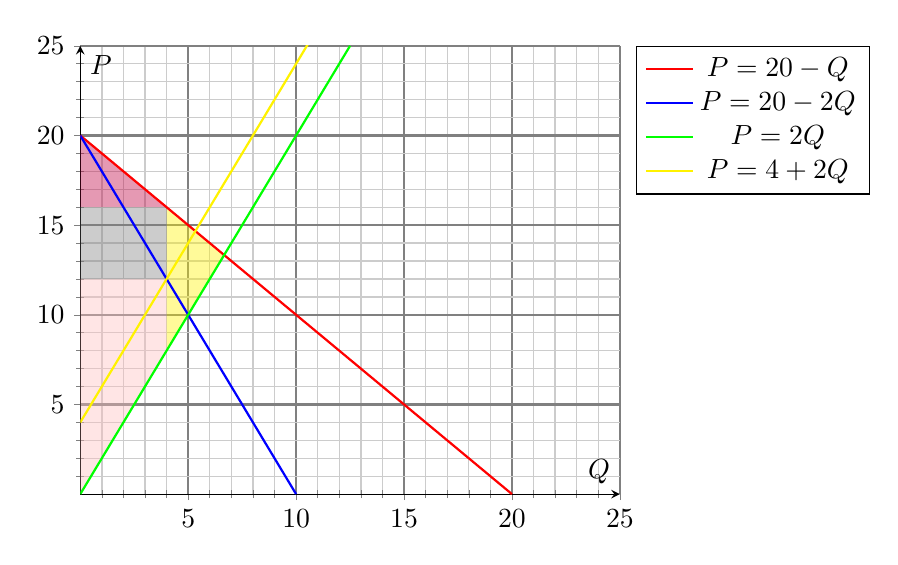
\begin{tikzpicture}
            \begin{axis}[
                axis lines=middle,
                xlabel={$Q$},
                ylabel={$P$},
                xmin=0, xmax=25,
                ymin=0, ymax=25,
                grid=both,
                minor tick num=4, 
                major grid style={line width=0.8pt,draw=black!50},
                minor grid style={line width=0.5pt,draw=black!20},
                legend pos=outer north east
            ]
            \fill[pink, opacity=0.4] (axis cs:0,12) -- (axis cs:4,12) -- (axis cs:4,8) -- (axis cs:0,0) -- cycle;
            
            \fill[purple, opacity=0.4] (axis cs:0,16) -- (axis cs:0,20) -- (axis cs:4,16) -- cycle;
            
            \fill[yellow, opacity=0.4] (axis cs:4,16) -- (axis cs:4,8) -- (axis cs:6.67,13.34) -- cycle;

            \fill[gray, opacity=0.4] (axis cs:0,16) -- (axis cs:0,12) -- (axis cs:4,12) -- (axis cs:4,16) -- cycle;
            
            \addplot[red, thick, domain=0:20] {20 - x};
            \addlegendentry{$P=20-Q$}
            \addplot[blue, thick, domain=0:10] {20 - 2*x};
            \addlegendentry{$P=20-2Q$}
            \addplot[green, thick, domain=0:12.5] {2*x};
            \addlegendentry{$P=2Q$}
            \addplot[yellow, thick, domain=0:15] {4 + 2*x};
            \addlegendentry{$P=4+2Q$}
            \end{axis}
        \end{tikzpicture}
        \end{center}
        \begin{itemize}
            \item Consumer Surplus = \(\frac{1}{2}\) $\times$ (20-16) $\times$ (4-0) = 8 $\Rightarrow \Delta CS=-4.5$ \\
            \item Producer Surplus = \(\frac{1}{2}\) $\times$ [(12-0)+(12-8)] $\times$ (4-0) = 32 $\Rightarrow \Delta PS=-18$ \\
            \item Deadweight Loss = \(\frac{1}{2}\) $\times$ (16-8) $\times$ (6.67-4) = 10.67 $\Rightarrow \Delta DWL= 6.5$
        \end{itemize} 
    \item 
        From Part B, Question 4, we know the demand and supply functions are as follows \\ $Q^d = -1.28P+22.4$ and $Q^s = 1.6P+8$ \\
        i.e. $P = -0.78125Q^d + 17.5$ and $P = 0.625Q^s - 5$ \\
        A 10\% rightward shift implies the new inverse demand function is
        $P=-0.78125Q^d + 19.25$ \\
        Equating this to the original inverse supply function $\Rightarrow$
        $-0.78125Q^d + 19.25 = 0.625Q^s - 5$ \\
        Thus, $P^* = \$5.78$ and $Q^* = 17.24$ units.
    \item
        \begin{enumerate}[label=(\roman*)]
            \item
                According to the tangency condition
                \[
                \frac{MU_x}{MU_y} = \frac{P_x}{P_y}
                \]
                $MU_x=\frac{x}{\sqrt{x^2+y^2}}$ , $MU_y=\frac{y}{\sqrt{x^2+y^2}}$ , $P_x=3$ , $P_y=4$ $\Rightarrow x=\frac{3y}{4}$\\
                Substituting this into the budget constraint $3x+4y=50$, we get $y=8$ and $x=6$\\
                $\therefore$ (6,8) is the optimal consumption bundle.
            \item 
                The above calculated bundle provides a utility of $\sqrt{6^2+8^2} = 10$. The indifference curve for this level of utility would be given by $\sqrt{x^2+y^2} =10$ and can be plotted along with the budget constraint as shown. 
                \begin{center}
                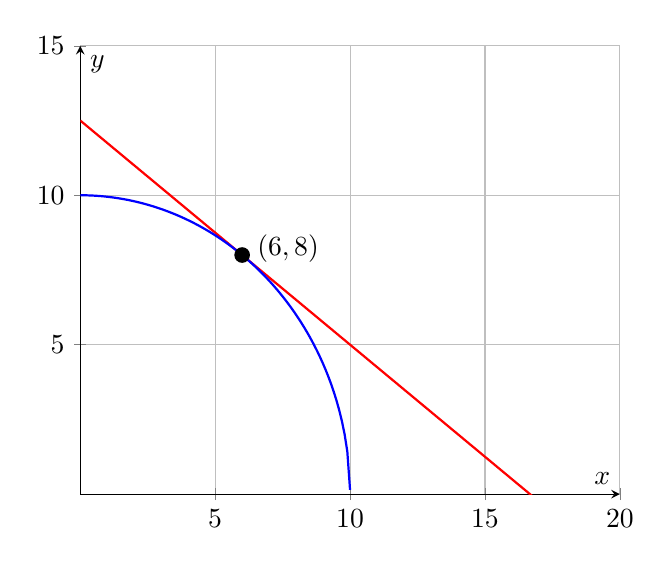
\begin{tikzpicture}
                    \begin{axis}[
                        axis lines=middle,
                        xlabel=$x$, ylabel=$y$,
                        xmin=0, xmax=20,
                        ymin=0, ymax=15,
                        grid=major,
                        ]
                        \addplot[domain=0:20, samples=100, red, thick] { (50 - 3*x)/4 };
                        \addplot[domain=0:10, samples=100, blue, thick] { sqrt(100 - x^2) };
                        \node[fill=black, circle, inner sep=2pt] at (axis cs:6,8) {};
                        \node[anchor=west] at (axis cs:6.2,8.2) {$(6,8)$};
                    \end{axis}
                \end{tikzpicture}
                \end{center}
                The indifference curve lies entirely underneath the budget constraint. Thus the utility can be increased till the curve is entirely above the line and just touches it at one point. Given the shape of the indifference curve, this happens at one of the corner points.\\
                Since the budget line's x-intercept $>$ y-intercept, utility would be maximized when the budget constraint and indifference curve meet at the x axis.\\
                \begin{minipage}{0.49\textwidth}
                    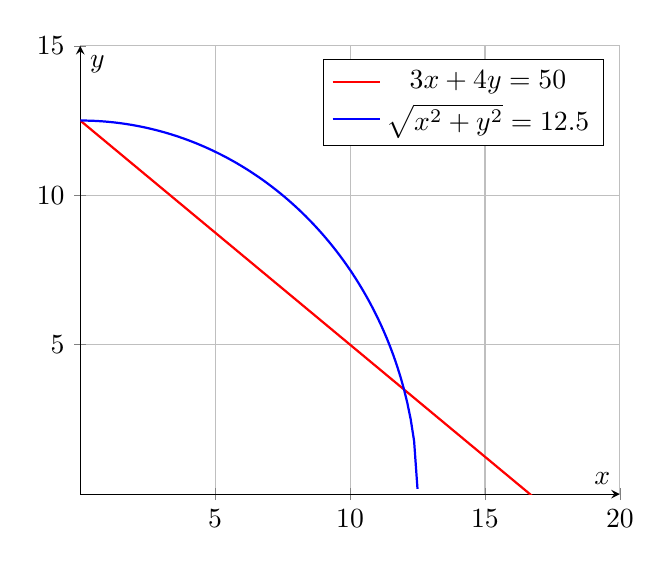
\begin{tikzpicture}
                    \begin{axis}[
                        axis lines=middle,
                        xlabel=$x$, ylabel=$y$,
                        xmin=0, xmax=20,
                        ymin=0, ymax=15,
                        grid=major,
                        legend pos=north east
                        ]
                        \addplot[domain=0:20, samples=100, red, thick] { (50 - 3*x)/4 };
                        \addlegendentry{$3x+4y=50$}
                        \addplot[domain=0:12.5, samples=100, blue, thick] { sqrt(156.25 - x^2) };
                        \addlegendentry{$\sqrt{x^2+y^2}=12.5$}
                    \end{axis}
                \end{tikzpicture}
                \end{minipage}
                \hfill
                \begin{minipage}{0.49\textwidth}
                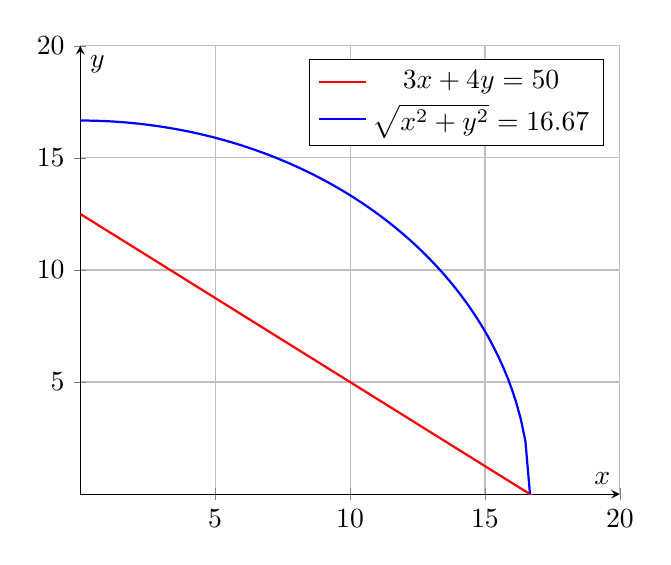
\begin{tikzpicture}
                    \begin{axis}[
                        axis lines=middle,
                        xlabel=$x$, ylabel=$y$,
                        xmin=0, xmax=20,
                        ymin=0, ymax=20,
                        grid=major,
                        legend pos=north east
                        ]
                        \addplot[domain=0:20, samples=100, red, thick] { (50 - 3*x)/4 };
                        \addlegendentry{$3x+4y=50$}
                        \addplot[domain=0:16.667, samples=100, blue, thick] { sqrt(277.777778 - x^2) };
                        \addlegendentry{$\sqrt{x^2+y^2}=16.67$}
                    \end{axis}
                \end{tikzpicture}
                \end{minipage}
                Therefore, the optimal consumption bundle is $(16.67,0)$ which gives a utility of 16.67, clearly greater than what we obtained from the consumption bundle calculated in part (i). 
        \end{enumerate} 
    \item 
        From tangency condition, we obtain 
        \[
        \frac{MU_{x_1}}{MU_{x_2}} =\frac{p_1}{p_2} \Rightarrow \frac{\alpha}{\beta} \cdot \frac{x_2}{x_1} = \frac{p_1}{p_2} \Rightarrow \frac{\alpha}{\beta} = \frac{p_1x_1}{p_2x_2} \Rightarrow \frac{\alpha + \beta}{\beta} = \frac{M}{p_2x_2}
        \]
        Therefore, $x_2^*$ = \(\frac{\beta}{\alpha + \beta} \cdot \frac{M}{p_2}\) \\
        Similarly, $x_1^*$ = \(\frac{\alpha}{\alpha + \beta} \cdot \frac{M}{p_1}\) \\
        \\
        Substituting these back into the utility function 
        \[
        U(x_1^*,x_2^*) = {(\frac{\alpha}{\alpha + \beta})}^\alpha \cdot {(\frac{\beta}{\alpha + \beta})}^\beta \cdot \frac{M^{\alpha + \beta}}{p_1^\alpha p_2^\beta}
        \]
    \item 
        From tangency condition we have 
        \[
        \frac{MP_K}{MP_L} = \frac{r}{w} \Rightarrow \frac{2L}{5K} = \frac{12}{5} \Rightarrow L=6K
        \]
        Since $Q=150 \Rightarrow 4K^\frac{2}{7}(6K)^\frac{5}{7}=150$\\
        Solving this gives $K=10.43$ and $L = 62.57$
    \item 
        Expected value of the demand curve (D) is given by
        \[
        E(D)=P(D_1)\cdot D_1 + P(D_2)\cdot D_2 \Rightarrow E(D) = (0.45)(450-0.58Q)+(0.55)(350-0.85Q) \Rightarrow E(D)=395-0.7285Q 
        \]
        Therefore, the expected demand curve is given by $P=395-0.7285Q$ \\
        $TR=395Q-0.7285Q^2 \Rightarrow MR=395-1.457Q$ and $MC=80$\\
        Profits maximized when $MR=MC \Rightarrow Q=216.2$ units.
    \item 
        Point price elasticity of demand is given by 
        \[
        \epsilon_p = \frac{\partial{Q}}{\partial{P}} \cdot \frac{P}{Q}
        \]
        $\therefore \epsilon_p = -abP^{-b-1}\times \frac{P}{Q} = -abP^{-b-1}\times \frac{P}{aP^{-b}} \Rightarrow \epsilon_p = -b$ \\
        Thus, if price decreased by 10\%, the quantity demanded has increased by 10b\%.
\end{enumerate}

\end{document}
